\subsection{Pulse generator} \label{subsec:Pulse_Generator} 
The read/write process described in section \refq{subsec:Sample_Memory} requires 4 CLK cycles to cycle all the way through the finite state machine that can write, or read, a single byte to the SRAM. These clocks are controlled by the Memory Distribution Module described in section \refq{subsec:Sample_Memory_Distribution} and this module must know when the 4 CLKs have been produced for byte 1 before it moves on and produces the CLKs for byte 2. This can seen in appendix \refq{App:MemoryDistributionCode} and will not be detailed here. The ADCs will require 16 CLKs and close timing of the digital control signals to function properly, so, several modules have a need to generate \textit{n} amount of CLKs for various purposes. A pulse generator module was made that can generate a desired amount of CLKs from a higher frequency master CLK signal and generate an output that can be checked to see when the CLKs are finished.

The full code listing for this can be seen in appendix \refq{App:PulseGeneratorCode}. The pulse generator starts when it sees a rising edge on a \textit{trigger} input as shown in listing \refq{lst:A_PulseGeneratorCode_Trigger} and is asynchronously reset when it gets a \textit{done} signal.

\lstinputlisting[language=C ,style = c,firstnumber=1, linerange=68-75, caption={VHDL code triggering the pulse generator}, label={lst:A_PulseGeneratorCode_Trigger}]{Sections/7_SystemDesign/Code/pulse_train_gen.vhd}

When the pulse generator is triggered it will start a counter that, for every rising edge of the master CLK, will increment a counter variable as shown in listing \refq{lst:A_PulseGeneratorCode_Counter} until it reaches a desired \textit{NR\_OF\_CLKs} as shown in line 5.

\lstinputlisting[language=C ,style = c,firstnumber=1, linerange=77-94, caption={VHDL code for a counter synchronous with a master CLK signal}, label={lst:A_PulseGeneratorCode_Counter}]{Sections/7_SystemDesign/Code/pulse_train_gen.vhd}

When the counter has reached \textit{NR\_OF\_CLKs}, the trigger process in listing \refq{lst:A_PulseGeneratorCode_Trigger} gets reset by the \textit{done} signal. The generate\_ram\_clks process in listing \refq{lst:A_PulseGeneratorCode_Counter} will control an \textit{active} signal that is used to control a process that gates a master CLK signal for as long as the counter isn't finished counting. This signal is used to control the master CLK gate process shown in listing \refq{lst:A_PulseGeneratorCode_Gate}.

\lstinputlisting[language=C ,style = c,firstnumber=1, linerange=111-124, caption={VHDL code for the master CLK gating process}, label={lst:A_PulseGeneratorCode_Gate}]{Sections/7_SystemDesign/Code/pulse_train_gen.vhd}

The process in listing \refq{lst:A_PulseGeneratorCode_Gate} will, for as long as active = '1' as shown in line 5, set the gate variable to '1'. The gate variable itself is used to gate the master CLK signals as shown in line 14. The gate\_output signal is AND'ed with the master CLK signal and the CLK signal will pass through to the pulse\_output signals for as long as active = '1'. The gating process gets stopped when the counter has reacher NR\_OF\_CLKs with the stop\_detect process shown in listing \refq{lst:A_PulseGeneratorCode_GateStop}.

\lstinputlisting[language=C ,style = c,firstnumber=1, linerange=96-109, caption={VHDL code for stopping the gate process}, label={lst:A_PulseGeneratorCode_GateStop}]{Sections/7_SystemDesign/Code/pulse_train_gen.vhd}

The stop process in listing \refq{lst:A_PulseGeneratorCode_GateStop} is falling edge triggered of the same master CLK used in the counter in listing \refq{lst:A_PulseGeneratorCode_Counter}. If the counter has reached NR\_OF\_CLKs the process will set the stop condition for the gate process in listing \refq{lst:A_PulseGeneratorCode_Gate}.

The result from all of these processes is that a single variable can be used to set the desired amount of output pulses from the module and the \textit{active} signal can be used in other modules to check when the pulse generation is complete. The output from this module can be seen in figure \refq{fig:7_2_7_PulseGenOutput}.

\begin{figure}[H]
    \centering
    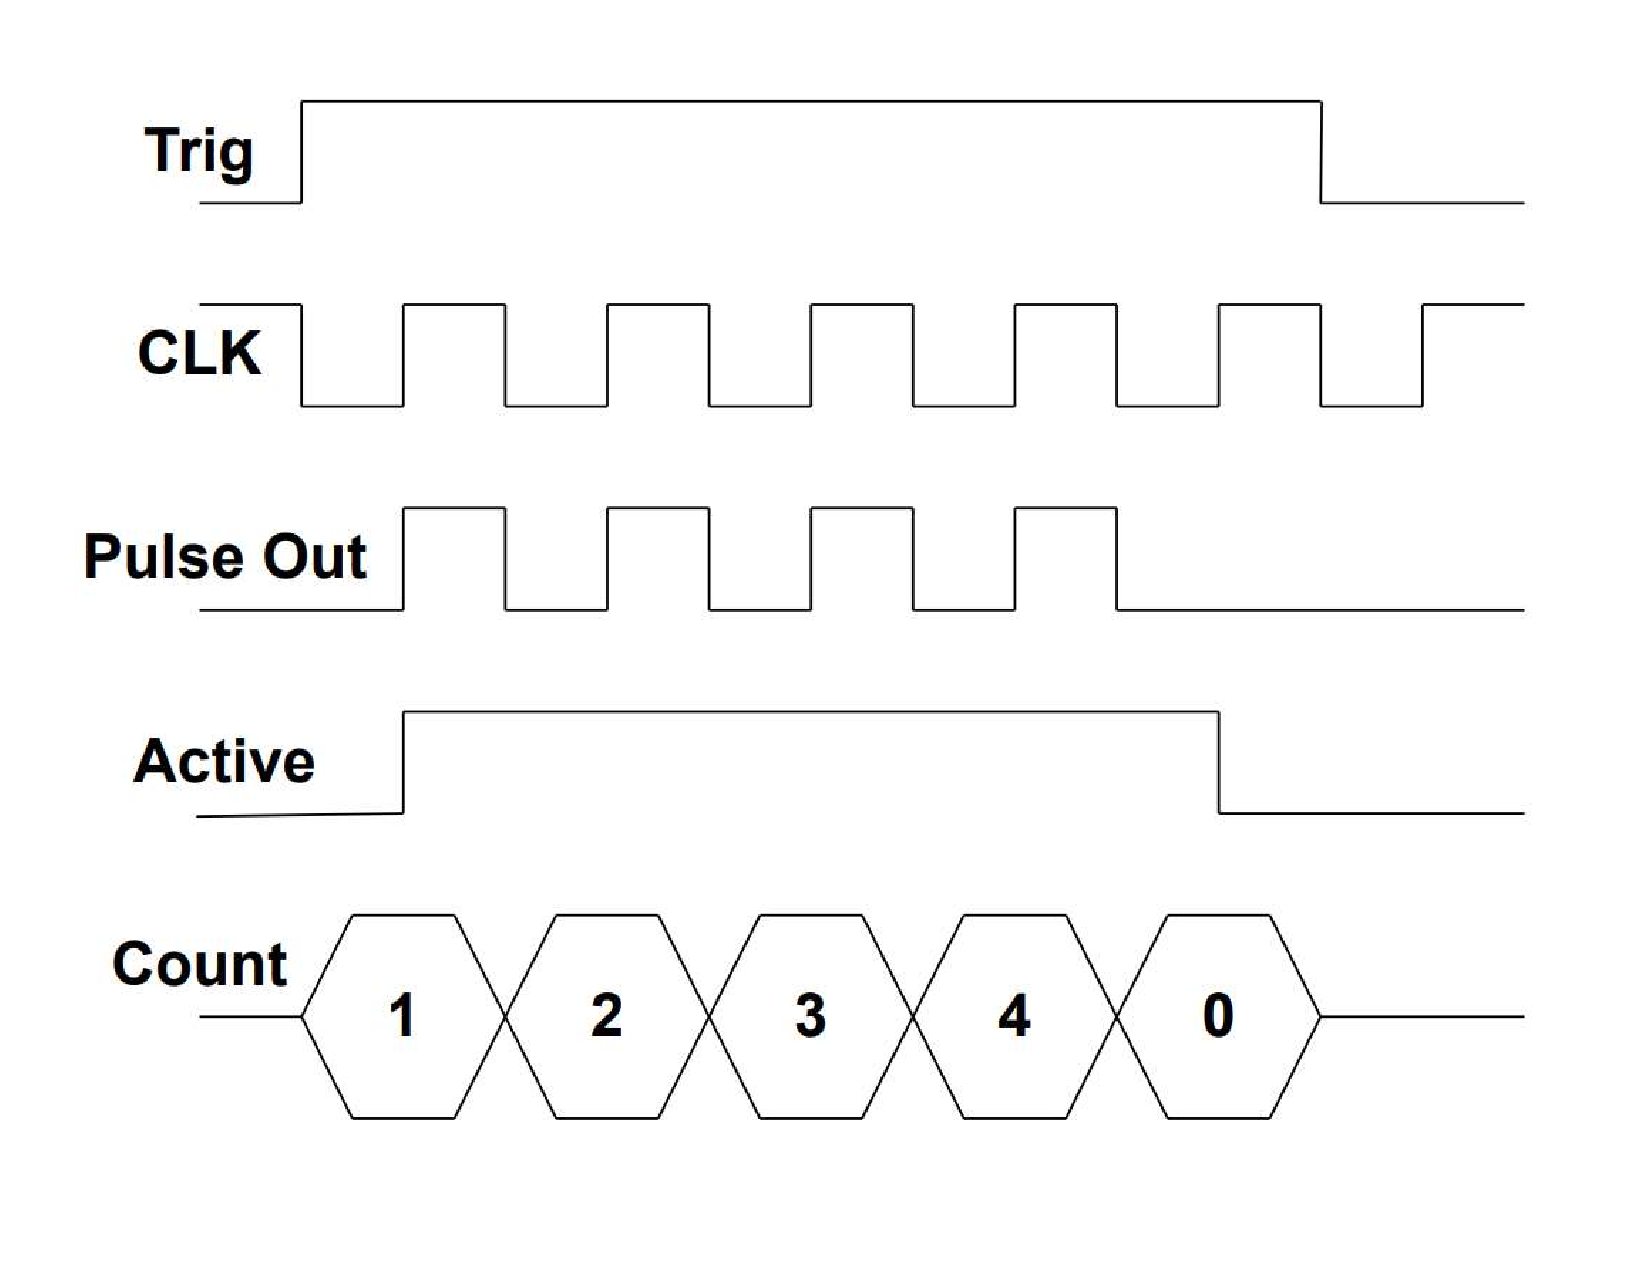
\includegraphics[clip, trim=0 50 0 0, width=0.68\textwidth]{Sections/7_SystemDesign/Figures/7_2_7_PulseGenOutput.pdf}
    \caption{A complete cycle of the pulse generator. The example is the output for NR\_OF\_CLKS = 4.}
    \label{fig:7_2_7_PulseGenOutput}
\end{figure}

As can be seen on figure \refq{fig:7_2_7_PulseGenOutput} the pulse generator will increment until NR\_OF\_CLKs has been reached and then reset for the next trigger input. The \textit{Active} signal mentioned earlier can be used from other modules to check if the pulse generator is finished.

A test of this pulse generator can be seen in appendix \refq{App:PulseGen}.